% !TeX program = XeLaTeX
%
% 为了得到最佳的排版结果,可以考虑安装免费的思源宋体、思源黑体与 Fandol 字库
% 思源字库可以前往 https://www.google.com/get/noto/help/cjk/ 下载
% 请安装 Language-specific OpenType/CFF (OTF) 的简体中文 SC 版本
% Fandol 字库可以通过发行版 TeX Live 或 MiKTeX 安装
% 如果已经安装了思源、Fandol 字库,请在导言区取消注释 9 处代码
%
\documentclass[
  zihao=5,
% 如果已经安装了思源、Fandol 字库,请取消注释下面一行代码
%  fontset=none,
  no-math,a4paper]{ctexart}
\frenchspacing
\ctexset{
  section={
    name={第,节},
    aftername=\hskip\ccwd\relax,
    format=\Large\bfseries
  },
  subsection/aftername=\hskip\ccwd\relax,
  subsubsection/aftername=\hskip\ccwd\relax
}
\renewcommand\sectionmark[1]{%
  \markright{%
    \normalfont\sffamily
    \CTEXifname{\CTEXthesection\hskip\ccwd\relax}{}#1%
  }%
}
\usepackage{mathtools}
\setmainfont{TeX Gyre Pagella}[
% 如果已经安装了思源、Fandol 字库,请取消注释下面两行代码
%  Scale=1.0534682080924855,
%  WordSpace={0.8984910836762689,1.2030178326474623,0.6954732510288066},
  SmallCapsFeatures={LetterSpace=5}
]
\setsansfont{TeX Gyre Heros}[
% 如果已经安装了思源、Fandol 字库,请取消注释下面两行代码
%  Scale=1.0054869684499314,
%  WordSpace={0.7887463562574224,1.4225072874851551,0.3662390687722673}
]
% 如果已经安装了思源、Fandol 字库,请取消注释下面设置西文等宽字体的四行代码
%\setmonofont{Noto Sans Mono CJK SC}[
%  BoldFont=Noto Sans Mono CJK SC Bold,
%  CharacterWidth=Half
%]
\usepackage[math-style=ISO]{unicode-math}
\setmathfont{TeX Gyre Pagella Math}[
% 如果已经安装了思源、Fandol 字库,请取消注释下面一行代码
%  Scale=1.0534682080924855
]
% 如果已经安装了思源、Fandol 字库,请取消注释下面设置中文字体的 35 行代码
%\setCJKmainfont{Noto Serif CJK SC}[
%  SizeFeatures={
%    {Size=-9,Font=Noto Serif CJK SC Medium},
%    {Size=9-}},
%  ItalicFont=FandolKai-Regular,
%  ItalicFeatures={FakeBold=1},
%  BoldFont=Noto Serif CJK SC Bold,
%  BoldItalicFont=FandolKai-Regular,
%  BoldItalicFeatures={FakeBold=3},
%  CharacterWidth=Full
%]
%\usepackage{etoolbox}
%\makeatletter
%\newcommand*\original@CJKsymbol{}
%\newcommand*\original@CJKpunctsymbol{}
%\let\original@CJKsymbol\CJKsymbol
%\let\original@CJKpunctsymbol\CJKpunctsymbol
%\newcommand*\raise@Fandol@CJK[1]{\raise0.08\ccwd\hbox{#1}}
%\appto\itshape{%
%  \let\CJKsymbol\raise@Fandol@CJK
%  \let\CJKpunctsymbol\raise@Fandol@CJK
%}
%\appto\upshape{%
%  \let\CJKsymbol\original@CJKsymbol
%  \let\CJKpunctsymbol\original@CJKpunctsymbol
%}
%\makeatother
%\setCJKsansfont{Noto Sans CJK SC}[
%  BoldFont=Noto Sans CJK SC Bold,
%  CharacterWidth=Full
%]
%\setCJKmonofont{Noto Sans Mono CJK SC}[
%  BoldFont=Noto Sans Mono CJK SC Bold,
%  CharacterWidth=Full
%]
\usepackage{zhlineskip}
\SetTextEnvironmentSinglespace{1.05}
\SetMathEnvironmentSinglespace{1.05}
% 如果已经安装了思源、Fandol 字库,请取消注释下面两行代码
%\SetTextEnvironmentSinglespace{1.106}
%\SetMathEnvironmentSinglespace{1.106}
\usepackage{caption}
\DeclareCaptionLabelSeparator{zhcolon}{~:}
\captionsetup{labelsep=zhcolon,format=hang}
\usepackage{enumitem}
\setlist{
  listparindent=\parindent,parsep=\parskip
}
\setlist[itemize,1]{
  itemsep=0pt,
  label=·,
% 如果已经安装了思源、Fandol 字库,请取消注释下面一行代码
%  label=・,
  leftmargin=\parindent,labelsep=0pt,labelwidth=0.5\parindent
}
\setlist[description,1]{
  font=\mdseries,
  leftmargin=\parindent,labelsep=0.5\parindent
}
\usepackage{booktabs}
\usepackage{hyperref}
\hypersetup{
  colorlinks=true,
  pdfstartview={FitH},
  unicode=true,
  pdftitle={zhlineskip-man},
  pdfauthor={张瑞熹}
}
\usepackage[open,openlevel=-1,numbered]{bookmark}
\usepackage[width=378bp]{geometry}

\makeatletter
% 如果已经安装了思源、Fandol 字库,请取消注释下面从 \ExplSyntaxOn
% 到 \ExplSyntaxOff 之间的 11 行代码
\ExplSyntaxOn
%\xeCJK_new_class:n { PoZheHao }
%\__xeCJK_save_CJK_class:n { PoZheHao }
%\xeCJK_declare_char_class:nn { PoZheHao } { "2014 }
%\seq_map_inline:Nn \g__xeCJK_class_seq
%  {
%    \str_if_eq:nnF {#1} { PoZheHao }
%      {
%        \xeCJK_copy_inter_class_toks:nnnn { PoZheHao } {#1} { FullRight } {#1}
%        \xeCJK_copy_inter_class_toks:nnnn {#1} { PoZheHao } {#1} { FullRight }
%      }
%  }
\ExplSyntaxOff
% From `doc.dtx'
\ifx\l@nohyphenation\undefined
  \newlanguage\l@nohyphenation
\fi
\newcommand*\meta{}
\DeclareRobustCommand\meta[1]{%
     \ensuremath\langle
     \ifmmode \expandafter \nfss@text \fi
     {%
      \meta@font@select
      \edef\meta@hyphen@restore
        {\hyphenchar\the\font\the\hyphenchar\font}%
      \hyphenchar\font\m@ne
      \language\l@nohyphenation
      #1\/%
      \meta@hyphen@restore
     }\ensuremath\rangle
}
\def\meta@font@select{\itshape}
% From `ltxdoc.dtx'
\newcommand*\cmd[1]{\cs{\expandafter\cmd@to@cs\string#1}}
\def\cmd@to@cs#1#2{\char\number`#2\relax}
\newcommand*\cs{}
\DeclareRobustCommand\cs[1]{\texttt{\char`\\#1}}
\newcommand\marg[1]{%
  {\ttfamily\char`\{}\meta{#1}{\ttfamily\char`\}}}
\newcommand\oarg[1]{%
  {\ttfamily[}\meta{#1}{\ttfamily]}}
\newcommand\parg[1]{%
  {\ttfamily(}\meta{#1}{\ttfamily)}}
% My commands
\newcommand\cls[1]{{\normalfont\ttfamily#1}}
\newcommand\pkg[1]{{\normalfont\ttfamily#1}}
\newcommand\opt[1]{{\normalfont\ttfamily#1}}
\newcommand\env[1]{{\normalfont\ttfamily#1}}
\newcommand*\packagedependency[1]{%
  \mbox{\pkg{#1}~宏包:}\ignorespaces
}
\newcommand*\keyvalueitem[3][2.5]{%
  \item[\opt{#2}\hskip0.5\ccwd\relax\rlap{\meta{#3}}\hskip#1\ccwd\relax]%
  \hskip\z@ \@plus 0.25\ccwd \@minus 0.25\ccwd
  \ignorespaces
}
\newcommand*\usercmditem[3][3]{%
  \item[\cmd{#2}\rlap{\marg{#3}}\hskip#1\ccwd\relax]%
  \hskip\z@ \@plus 0.25\ccwd \@minus 0.25\ccwd
  \ignorespaces
}
\newcommand*\defaultleadingratio[3]{%
  \opt{#1} & $#2$ & $#3$%
}
\newcommand*\fontandsinglespaceratio[2]{%
  #1 & $#2$%
}
\newenvironment{originalpmatrix}{\left(\env@matrix}{\endmatrix\right)}
\newenvironment{originalcases}{\env@cases}{\endarray\right.}
\newcommand*\myemail{ruixizhang42@gmail.com}
\makeatother

\title{\vspace*{-18bp}\pkg{zhlineskip} 宏包}
\author{张瑞熹\thanks{\href{mailto:\myemail}{\nolinkurl{\myemail}}。}}
\date{2018/10/28\hskip\ccwd\relax v1.0c}

\begin{document}

\maketitle

\tableofcontents

\section{简介}

\pkg{zhlineskip} 宏包允许用户指定正文行距相比于正文字号的倍数(通常建议设置在
$1.5$ 至 $1.67$ 之间),以及脚注行距相比于脚注字号的倍数。另一方面,由于数学公式
主要是由西文字符构成的,\pkg{zhlineskip} 还能将数学公式的行距“恢复”成西文
较为紧凑的行距(通常为西文字号的 $1.2$~倍),使得全文的视觉密度较为均匀。最后,
本宏包还支持按照 Microsoft Word 进行“多倍行距”排版。

\subsection{宏包依赖}

本宏包是在 \CTeX\ 宏集大环境下设计出来的,目的是要分开处理中文与数学的行距。
如果你并没用 \CTeX\ 的文档类,那么不建议使用本宏包。\pkg{zhlineskip} 依赖于
下面这些宏包:
\begin{itemize}
\item \packagedependency{kvoptions}
为用户提供载入本宏包的键值选项。
\item \packagedependency{xintexpr~}
实现精确的浮点运算,属于 \pkg{xint} 宏集的一个部分。
\item \packagedependency{etoolbox~}
处理脚注行距与数学行距时需要打补丁。
\item \packagedependency{mathtools}
只有在恢复数学行距为西文行距时,才会载入这个宏包。
\end{itemize}
请确保你的 \TeX\ 发行版里已经安装好了以上这些宏包的最新版本。

\subsection{中西有别}

在西文排版里,相邻两行\emph{基线}(baseline)之间的距离称为\emph{行距}(leading,
发音为 led-ding)。这个词的词根是 lead,即\emph{铅}。早在铅字时代,每当工匠填满
一行铅字之后要开始填下一行,都会在两行之间插入铅条,从而适当地扩大行距。因为西文的
每个字母四周与其\emph{字框}(em-box,见图~\ref{fig:eng-font-size})之间有
较大的空隙,所以不需要插入很高的铅条。一般来说,西文的行距为\emph{字号}(font
size)的 $1.2$ 至 $1.45$~倍\footnote{参见
\url{https://practicaltypography.com/line-spacing.html}。}。

\begin{figure}[h]
\centering

\includegraphics{Latinmetrics}
\caption[西文字体]{西文字体。绿色方框即为 em-box,它在纸上的实际边长就是西文字号。}
\label{fig:eng-font-size}
\end{figure}

中文排版虽然没有基线的概念,但有非常相似的概念:\emph{底线}(ideographic baseline,
见图~\ref{fig:chi-font-size})。中文里相邻两行底线之间的距离,与西文里行距的
概念是一致的。另一概念是上一行底线和下一行\emph{顶线}之间的距离,即\emph{行间距}(line
gap),这与西文里插入铅条的高度是一致的。由于汉字四周与其字框间的空隙较小,所以需要
使用比西文更大的行间距。根据场合不同,行间距从字号的 $1/4$ 至 $1$~倍不等:以中文
书刊为例,行间距一般为字号的 $1/2$ 至 $2/3$~倍\footnote{参见张胜涛、王忆波著
《方正飞腾4.0实用培训教程》,第~6.1.1~节。},即行距约为字号的 $1.5$ 至 $1.67$~倍。

\begin{figure}[h]
\centering
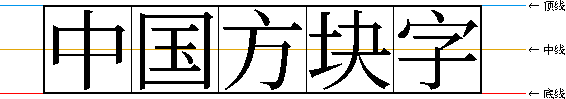
\includegraphics{CJKmetrics}
\caption[中文字体]{中文字体。汉字字面几乎占满整个字框,字框的边长即为中文字号。}
\label{fig:chi-font-size}
\end{figure}

在一般情况下,\CTeX\ 会默认用 \opt{linespread=1.3} 这个文档类选项将中文的
行距设置为字号的 $1.56$~倍(基础行距是字号的 $1.2$~倍,而 $1.2 \times 1.3
= 1.56$)。通过这种方法扩大全文的行距,自然会影响到文章里数学公式的行距。而数学
公式主要是由西文字符构成的,把它们按照中文的行距进行排版,就会显得有些松散。
图~\ref{fig:math-leading} 左边是 \CTeX\ 默认排版效果,文本、数学看似
一紧、一松;右边是配合用 \pkg{zhlineskip} 的效果,视觉密度比较均匀。
\pkg{zhlineskip} 宏包还允许用户调整数学行距的大小。

\begin{figure}[h]
\sbox0{%
\begin{minipage}[t]{162pt}
\fontsize{9}{10.8}\linespread{1.3}\selectfont
\rule{0pt}{\ht\strutbox}\hskip2\ccwd\relax
设 $\symbf{I}_2=\begin{psmallmatrix} 1&0\\0&1 \end{psmallmatrix}$.
又设 $\symbf{A}=(a_{ij})_{m \times n}$ 为一个 $m$~行 $n$~列的实值矩阵, 即
\[
\symbf{A} = \begin{originalpmatrix}
a_{11} & a_{12} & \dotsc & a_{1n} \\
a_{21} & a_{22} & \dotsc & a_{2n} \\
\vdots & \vdots &        & \vdots \\
a_{m1} & a_{m2} & \dotsc & a_{mn}
\end{originalpmatrix},
\]
其中 $a_{ij} \in \mathbb{R}$, $i=1,\dotsc,m$, $j=1,\dotsc,n$.
又因为
\[
\sum_{\substack{i=1\\i\neq j}}^m a_{ij} = \begin{originalcases}
0, & j=1,\\
1, & j>1,
\end{originalcases}
\]
我们得到……\rule[-\dp\strutbox]{0pt}{\dp\strutbox}
\end{minipage}%
}%
\centering
\rule[\dimexpr-\dp0-0.5em\relax]{0.4pt}{\dimexpr\dp0+\ht0+1em\relax}\quad
\copy0\quad
\rule[\dimexpr-\dp0-0.5em\relax]{0.4pt}{\dimexpr\dp0+\ht0+1em\relax}\quad
\begin{minipage}[t]{162pt}
\fontsize{9}{10.8}\linespread{1.25}\selectfont
\hskip2\ccwd\relax
设 $\symbf{I}_2=\begin{psmallmatrix} 1&0\\0&1 \end{psmallmatrix}$.
又设 $\symbf{A}=(a_{ij})_{m \times n}$ 为一个 $m$~行 $n$~列的实值矩阵, 即
\[
\symbf{A} = \begin{pmatrix}
a_{11} & a_{12} & \dotsc & a_{1n} \\
a_{21} & a_{22} & \dotsc & a_{2n} \\
\vdots & \vdots &        & \vdots \\
a_{m1} & a_{m2} & \dotsc & a_{mn}
\end{pmatrix},
\]
其中 $a_{ij} \in \mathbb{R}$, $i=1,\dotsc,m$, $j=1,\dotsc,n$.
又因为
\[
\sum_{\substack{i=1\\i\neq j}}^m a_{ij} = \begin{cases}
0, & j=1,\\
1, & j>1,
\end{cases}
\]
我们得到……
\end{minipage}\quad
\rule[\dimexpr-\dp0-0.5em\relax]{0.4pt}{\dimexpr\dp0+\ht0+1em\relax}%
\llap{\rule[\dimexpr-\dp0-0.5em\relax]{\dimexpr2\wd0+4em+1.2pt\relax}{0.4pt}}%
\llap{\rule[\dimexpr\ht0+0.5em-0.4pt\relax]{\dimexpr2\wd0+4em+1.2pt\relax}{0.4pt}}
\caption[数学行距对比]{数学行距对比。在左图中,大矩阵 \env{pmatrix} 与分类
  \env{cases} 两个环境受到影响,行距都被扩大了;但第一行文本里的小矩阵与末尾
  公式里求和号的下角标却没有受到影响,行距仍然较为紧凑。在右图中,数学公式的行距
  都是西文的行距,密度比较均匀,行间公式里的大括弧、大括号也不会特别突兀。}
\label{fig:math-leading}
\end{figure}

综上所述,在进行中西文混排时,最好能够区分中文与西文的行距。在使用 \pkg{zhlineskip}
时,就可以分开处理中文文本与数学公式的行距。用户甚至还能分别指定正文行距与脚注
行距,实现灵活的排版。同时,\pkg{zhlineskip} 宏包能够恢复各种“多行”数学环境
(包括矩阵、分类、多行公式推导等等)的行距,使数学行距符合西文行距的规范。

最后,\pkg{zhlineskip} 宏包还支持用户在一定范围内按 Microsoft Word 的
“多倍行距”进行排版\footnote{本宏包默认假定“被要求”用的字体是中易系列字体,
这包括 Microsoft Word 里的“宋体”、“黑体”、“楷体”与“仿宋”。若改用其他字体,
可能需要调整 \opt{MSWordSinglespaceRatio} 的值。
参见第~\ref{sec:key-value}~节与第~\ref{sec:MS-Word}~节。}。
用户可以指定“多倍行距”的“倍数”,但是这只保证用 \TeX\ 排出来的文本行距与用
Microsoft Word 排的行距相同。硬要用 \TeX\ 模仿 Microsoft Word 是没有
太大意义的。

\section{功能介绍}

首先,请避免使用“多倍行距”这个概念:Microsoft Word 中“单倍行距”的值严重依赖于
字体(参见第~\ref{sec:MS-Word}~节)。在严格排版的时候,一般都会给定具体的字号
与行距,例如字号 $12$~磅、行距 $22$~磅。对于一般的用户,指定目标行距相比字号的
倍数即可——\pkg{zhlineskip} 宏包可以自动提取基础行距(即 \TeX\ 中的单倍行距)
相比字号的倍数(详见表~\ref{tab:default-leading-ratio}),再通过用户指定的
倍数来计算所需的行伸展因子。
\begin{table}[h]
\centering
\caption[基础行距倍数]{\cls{ctexart} 与 \cls{article} 各个文档类选项
  设置的基础行距倍数。}
\label{tab:default-leading-ratio}
\begin{tabular}{l l l}
\toprule
文档类选项 & 正文基础行距 & 脚注基础行距 \\
\midrule
\defaultleadingratio{zihao=5}{1.2}{1.2} \\
\defaultleadingratio{zihao=-4}{1.2}{1.2} \\
\defaultleadingratio{10pt}{12/10}{9.5/8} \\
\defaultleadingratio{11pt}{13.6/10.95}{11/9} \\
\defaultleadingratio{12pt}{14.5/12}{12/10} \\
\bottomrule
\end{tabular}
\end{table}

\subsection{载入宏包时的键值选项}
\label{sec:key-value}

载入 \pkg{zhlineskip} 宏包时可以设定六个基本的键值选项,它们分别是:
\begin{description}
\keyvalueitem{bodytextleadingratio}{real}
指定正文目标行距相比于正文字号的倍数。以书刊为例,建议设置在~$1.5$ 至~$1.67$
之间。缺省值是~\opt{1.5},即 $1/2$~的行间距。
\keyvalueitem{footnoteleadingratio}{real}
指定脚注目标行距相比于脚注字号的倍数,它可以比正文的倍数稍小一些,建议设置在正文
倍数的 $98\%$ 至 $100\%$ 之间。缺省值是~\opt{1.48},即大约为正文倍数的~$98.67\%$。
\keyvalueitem{restoremathleading}{bool}
指定是否要将数学公式的行距恢复成西文基础行距。缺省值是~\opt{true},即恢复数学
行距。该选项为真时,会自动载入 \pkg{mathtools} 宏包,此时还能利用
\cmd{\SetMathEnvironmentSinglespace}\marg{real}
命令\emph{微调}数学公式的基础行距。
\keyvalueitem{UseMSWordMultipleLineSpacing}{bool}
在排版论文时,如果被要求按照 Microsoft Word 来设置“多倍行距”,那么用户可以
将该选项设置为~\opt{true},并通过设置 \opt{MSWordLineSpacingMultiple}
指定“倍数”,这会忽略用户之前指定的正文行距与脚注行距倍数,但是与数学行距的设置
独立。该选项的缺省值是~\opt{false}。
\keyvalueitem{MSWordLineSpacingMultiple}{real}
设置 Microsoft Word“多倍行距”的“倍数”,
仅在 \opt{UseMSWordMultipleLineSpacing} 为真时生效。
缺省值是~\opt{1.15},在不修改 \opt{MSWordSinglespaceRatio} 时,
相当于设置了目标行距为字号的 $1.49140625$~倍,适用于中易字体
(参见第~\ref{sec:MS-Word}~节)。
\keyvalueitem{MSWordSinglespaceRatio}{real}
设置 Microsoft Word 的“单倍行距”相比字号的倍数,
仅在 \opt{UseMSWordMultipleLineSpacing} 为真时生效。
缺省值是~\opt{1.296875},适用于中易字体(参见第~\ref{sec:MS-Word}~节)。
若改用其他字体,则需调整该选项的值。
\end{description}

\subsection{载入宏包后的用户命令}

\subsubsection{调整数学公式的行距}

当键值选项 \opt{restoremathleading} 为~\opt{true} 时,数学公式的行距被
恢复成字号的 $1.2$~倍。对于某些字面较大的数学字体(例如类似 Palatino 的字体),
这个基础行距会显得过小。此时,用户可以通过如下命令微调数学行距:
\begin{description}
\usercmditem{\SetMathEnvironmentSinglespace}{real}
如果数学字体来自 \pkg{newpxmath} 或是 TeX Gyre Pagella Math,那么
数学行距在字号 $1.2$~倍的基础上再扩大 $1.05$~倍更加合适。此时,只需指定
\verb|\SetMathEnvironmentSinglespace{1.05}| 即可。
\end{description}
本宏包恢复的多行数学环境包括:
\begin{description}
\raggedright
\item[\LaTeX\ 环境]
\env{array};
\item[\pkg{amsmath} 宏包各环境]
\env{matrix},
\env{pmatrix},
\env{bmatrix},
\env{Bmatrix},
\env{vmatrix},
\env{Vmatrix},
\env{cases},
\env{aligned},
\env{alignedat},
\env{gathered},
\env{gather},
\env{gather*},
\env{align},
\env{align*},
\env{flalign},
\env{flalign*},
\env{alignat},
\env{alignat*},
\env{xalignat},
\env{xalignat*},
\env{xxalignat},
\env{multline},
\env{multline*},
\env{split};
\item[\pkg{mathtools} 宏包各环境]
\env{matrix*},
\env{pmatrix*},
\env{bmatrix*},
\env{Bmatrix*},
\env{vmatrix*},
\env{Vmatrix*},
\env{cases*},
\env{dcases},
\env{dcases*},
\env{rcases},
\env{rcases*},
\env{drcases},
\env{drcases*},
\env{multlined},
\env{lgathered},
\env{rgathered}。
\end{description}
超出上述列表范围、用户自定义的\emph{数学}环境,可用如下命令恢复其行距:
\begin{description}
\usercmditem[6]{\RestoreMathEnvironmentLeading}{env name}
使用范例:本宏包恢复数学环境 \env{array} 的行距,通过
\verb|\RestoreMathEnvironmentLeading{array}| 实现。
\end{description}

\emph{注意,在 \opt{restoremathleading} 为~\opt{false} 时,
\cmd{\SetMathEnvironmentSinglespace}
与 \cmd{\RestoreMathEnvironmentLeading} 无效。}

\subsubsection{调整西文文本的行距}

与数学行距命令对应,本宏包还提供两个调整\emph{西文文本}行距的命令,用法类似。
\begin{description}
\usercmditem{\SetTextEnvironmentSinglespace}{real}
如果西文字体来自 \pkg{newpxtext} 或是 TeX Gyre Pagella,那么可以指定
\verb|\SetTextEnvironmentSinglespace{1.05}|。
\usercmditem[6]{\RestoreTextEnvironmentLeading}{env name}
使用范例:假设文中的表格仅含西文、数字,此时如果想要文本环境 \env{tabular} 的
行距与西文行距一致,可通过
\verb|\RestoreTextEnvironmentLeading{tabular}| 实现。
\end{description}

如果作者没有顾及到某些\emph{基本环境}(数学或文本),鼓励用户向 \pkg{zhlineskip} 的
\href{https://github.com/CTeX-org/ctex-kit/issues}{GitHub 维护页}%
提供相关信息。

\subsection{使用范例}

下面以 \CTeX\ 提供的 \cls{ctexart} 文档类为例,展示 \pkg{zhlineskip} 的
使用方法。

\subsubsection*{例:直接载入}

\begin{verbatim}
    \documentclass{ctexart}
    \usepackage{zhlineskip}
    \begin{document}
    正文测试。
    \end{document}
\end{verbatim}

\subsubsection*{例:设置正文行距为字号的 1.6~倍}

\begin{verbatim}
    \documentclass{ctexart}
    \usepackage[
        bodytextleadingratio=1.6, % 设置正文行距倍数为 1.6
        footnoteleadingratio=1.57 % 设置脚注行距倍数为 1.57
      ]{zhlineskip}               % 缺省数学行距倍数为 1.2
    \begin{document}
    正文测试。
    \end{document}
\end{verbatim}

\subsubsection*{例:按照 Microsoft Word 设置“1.62~倍行距”}

\begin{verbatim}
    \documentclass{ctexart}
    \usepackage[
        restoremathleading=false,
        UseMSWordMultipleLineSpacing,
        MSWordLineSpacingMultiple=1.62
      ]{zhlineskip}
    \begin{document}
    按照 Microsoft Word 设置 1.62~倍行距。
    \end{document}
\end{verbatim}

\subsubsection*{例:中文正文里需要插入成段的西文}

如果插入的西文是引用参考文献的段落,那么使用 \env{quote} 或 \env{quotation}
环境就比较合适。此时,可以直接在引用环境内部使用 \cmd{\linespread}\marg{real}
命令,建议将 \meta{real} 设置在正文行距倍数的 $0.7$~倍左右。例如,在载入
\pkg{zhlineskip} 宏包后,正文行距为字号的 $1.5$~倍,那么
\verb|\linespread{1.05}| 就比较合适($1.5 \times 0.7 = 1.05$)。
\begin{verbatim}
    \documentclass{ctexart}
    \usepackage{zhlineskip}
    \begin{document}
    下面引用一段出自英文文献的段落:
    \begin{quotation}
    \linespread{1.05}\selectfont % 此处数值为正文行距倍数的 0.7 倍左右
    A quotation from English literature.
    \end{quotation}
    \end{document}
\end{verbatim}

\subsection{Microsoft Word 中的“单倍行距”}
\label{sec:MS-Word}

Microsoft Word 中“单倍行距”的设置,其行距值相比字号的倍数严重依赖于字体。
表~\ref{tab:word-line-height} 列出几种常用字体对应的倍数。正是因为“单倍
行距”本身随着字体而变化,所以请尽量避免使用“多倍行距”的概念!
\begin{table}[h]
\centering
\caption[单倍行距倍数]{在 Microsoft Word 中设置“单倍行距”后,实际的行距
  依赖于字体。}
\label{tab:word-line-height}
\begin{tabular}{l l}
\toprule
字体名称 & “单倍行距”除以字号的倍数 \\
\midrule
\fontandsinglespaceratio{Arial}{2355/2048=1.14990234375} \\
\fontandsinglespaceratio{Times New Roman}{2355/2048=1.14990234375} \\
\fontandsinglespaceratio{中易系列字体}{\phantom0332/256\phantom0=1.296875} \\
\fontandsinglespaceratio{思源宋体}{1869/1000=1.869} \\
\fontandsinglespaceratio{思源黑体}{1924/1000=1.924} \\
\bottomrule
\end{tabular}
\end{table}

\begin{thebibliography}{9}
\bibitem{butterick2018linespacing}
\textsc{Butterick, Matthew}.
\newblock \textit{Butterick's Practical Typography\textup:
  Line spacing}.
\newblock \url{https://practicaltypography.com/line-spacing.html},
  访问日期: 2018/10/28.

\bibitem{knuth1986tex}
\textsc{Knuth, Donald Ervin}.
\newblock \textit{The \TeX book}.
\newblock Addison--Wesley, 1986.

\bibitem{lunde2008cjkv}
\textsc{Lunde, Ken}.
\newblock \textit{CJKV Information Processing\textup:
  Chinese\textup, Japanese\textup, Korean \textup\&
  Vietnamese Computing} (2~ed.).
\newblock O'Reilly Media, Inc., 2008.

\bibitem{zhang2005fang}
\textsc{张胜涛, 王忆波}.
\newblock \textit{方正飞腾4.0实用培训教程}.
\newblock 清华大学出版社, 2005.
\end{thebibliography}

\end{document}